\documentclass[../main.tex]{subfiles}
\begin{document}

In this section, we will only be talking about convex polytopes.

\subsection{Regular polytopes and finite Coxeter groups}

As we've seen already, the symmetry groups of regular polytopes are Coxeter groups. Thus we can define a map from regular polytopes to finite Coxeter groups, based on their symmetries.\newline

\noindent\textbf{Definition 5.1.1.} If a polytope's symmetry group is a Coxeter, we say the polytope is \textit{defined by} that Coxeter group. Similarly, this Coxeter group \textit{defines} the polytope.\newline

Naturally, we can ask: Is this map a bijection? We know that dual polyhedra have the same symmetries, so clearly the answer is no. In fact, every polytope has the same symmetry group - and hence is defined by the same Coxeter group - as its dual. This clearly shows that the map is not injective and so is not a bijection. But the question remains, is the map surjective? That is to say, does every finite Coxeter group define a regular polytope? The answer to this question is also no, but why?

For this, we make use of the fact that no two Coxeter groups can be define the same polytope. This is clear since all Coxeter groups are unique. Because of this, we can refer to the Coxeter group that defines a given polytope as the polytope's Coxeter group. With this, we only need to show that there are more Coxeter groups than regular polytopes.\newline

\noindent\textbf{Lemma 5.1.2.} For $k \geq 5$, there are only 3 regular convex $k$-polytopes. Specifically, these are the $k$-simplex, the $k$-cube, and its dual, the $k$-orthoplex.\cite{Coxeter1973}\newline

\noindent\textbf{Proposition 5.1.3.} The map from regular polytopes to finite Coxeter groups is not surjective.
\begin{proof}
    We will use the fact that a Coxeter group $C_k$ defines a $k$-polytope. This $k$ is the number of generators of $C_k$, or, equivalently, the number of nodes in its Coxeter diagram.
    
    For $k = 5$, there are $3$ Coxeter groups: $A_5$, $BC_5$, and $D_5$. From Lemma 5.1.2, we know that there are $3$ regular $5$-polytopes. At first glance this seems fine, but remember that duals are defined by the same Coxeter group, meaning there are only $2$ unique symmetry groups of regular $5$-polytopes. Hence, one of the $3$ Coxeter groups does not define a regular polytope, and so the map is not surjective.
\end{proof}

\noindent\textbf{Remark 5.1.4.} With some work, you can find that $A_5$ defines the $5$-simplex and $BC_5$ defines both the $5$-cube and $5$-orthoplex, and so $D_5$ does not define a regular polytope. This is actually true for any number of dimensions; $A_n$ defines the $n$-simplex and $BC_n$ defines the $n$-cube and $n$-orthoplex.\newline

This means that $D_n, \forall n\geq5$ as well as $E_6$, $E_7$ and $E_8$  do not define regular polytopes. This begs the question: Which polytopes are defined by the remaining groups? To answer this, we need to introduce a new category of polytope.

\subsection{Uniform polytopes}

\noindent\textbf{Definition 5.2.1.} A polytope is \textit{$k$-face-transitive} if its symmetry group acts transitively on the $k$-faces on the polytope.\newline

\noindent\textbf{Remark 5.2.2.} Regular $k$-polytopes are $j$-face-transitive $\forall j<k$.\newline

\noindent\textbf{Definition 5.2.3.} A polytope is \textit{uniform} if it is vertex-transitive and has uniform facets. Uniform polygons are defined as regular polygons\footnote{This disallows polygons (and by extension polytopes) having edges of different lengths.}.\newline

This new category of polytopes contains the polytopes defined by $D_n$, $E_6$, $E_7$ and $E_8$, as well as many more, so let's create a way to differentiate them based on their symmetries.

\subsection{Extended Coxeter diagrams}

We can extend the Coxeter diagram to include more information about the specific polytope that it defines. Because of this, extended Coxeter diagrams do not represent unique Coxeter groups, but rather unique polytopes.\newline

\noindent\textbf{Definition 5.3.1.} The \textit{fundamental domain} of a uniform polytope is the\footnote{There are multiple regions that fit this definition, but for our purposes they are all equivalent (the polytope's Coxeter group acts transitively on the domain), so we can refer to it as the fundamental domain.} connected region containing exactly one point from each orbit of the points on the boundary of the polytope under its symmetry group. This can be visualised as the smallest region on the boundary of the polytope bounded by the planes of reflection of its Coxeter group.\newline

\begin{figure}[!h]
\centering
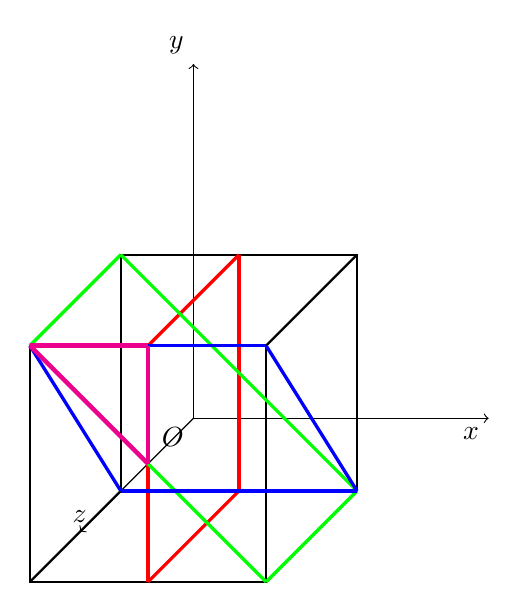
\begin{tikzpicture}[scale=1.5]

\draw[->] (0,0,0) -- (2.5,0,0) node[anchor=north east]{$x$};
\draw[->] (0,0,0) -- (0,3,0) node[anchor=south east]{$y$};
\draw[->] (0,0,0) -- (0,0,2.5) node[anchor=south]{$z$};


\def\s{1}


\draw[thick] (-\s,-\s,-\s) -- (\s,-\s,-\s) -- (\s,\s,-\s) -- (-\s,\s,-\s) -- cycle;

\draw[thick] (-\s,-\s,\s) -- (\s,-\s,\s) -- (\s,\s,\s) -- (-\s,\s,\s) -- cycle;

\foreach \x in {-1,1} {
  \foreach \y in {-1,1} {
    \draw[thick] (\x,\y,-1) -- (\x,\y,1);
  }
}

\draw[very thick, red] (0,1,1) -- (0,1,-1);
\draw[very thick, red] (0,1,-1) -- (0,-1,-1);
\draw[very thick, red] (0,-1,-1) -- (0,-1,1);
\draw[very thick, red] (0,-1,1) -- (0,1,1);

\draw[very thick, green] (-1,1,1) -- (-1,1,-1);
\draw[very thick, green] (-1,1,-1) -- (1,-1,-1);
\draw[very thick, green] (1,-1,-1) -- (1,-1,1);
\draw[very thick, green] (1,-1,1) -- (-1,1,1);

\draw[very thick, blue] (-1,1,1) -- (1,1,1);
\draw[very thick, blue] (1,1,1) -- (1,-1,-1);
\draw[very thick, blue] (1,-1,-1) -- (-1,-1,-1);
\draw[very thick, blue] (-1,-1,-1) -- (-1,1,1);

\draw[ultra thick, magenta] (-1,1,1) -- (0,1,1);
\draw[ultra thick, magenta] (0,1,1) -- (0,0,1);
\draw[ultra thick, magenta] (0,0,1) -- (-1,1,1);

\node[below left] at (0,0,0) {\(O\)};
\end{tikzpicture}
\caption{The fundamental domain of a cube}
\end{figure}

\noindent\textbf{Definition 5.3.2.} The \textit{generating vertex} of a uniform polytope is the vertex that lies in its fundamental domain.\newline

\begin{figure}[!h]
\centering
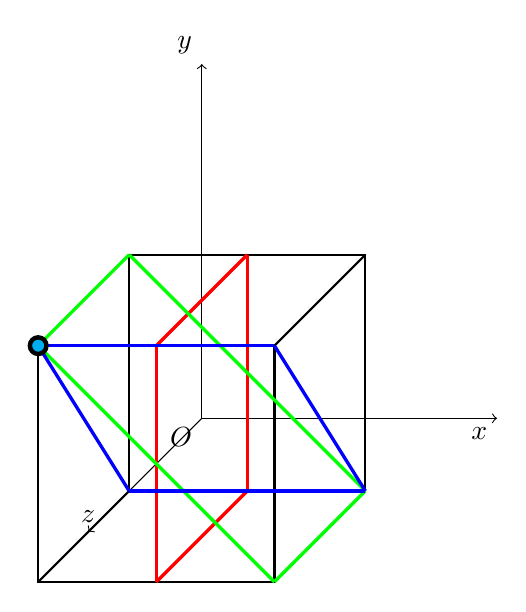
\begin{tikzpicture}[scale=1.5]

\draw[->] (0,0,0) -- (2.5,0,0) node[anchor=north east]{$x$};
\draw[->] (0,0,0) -- (0,3,0) node[anchor=south east]{$y$};
\draw[->] (0,0,0) -- (0,0,2.5) node[anchor=south]{$z$};


\def\s{1}


\draw[thick] (-\s,-\s,-\s) -- (\s,-\s,-\s) -- (\s,\s,-\s) -- (-\s,\s,-\s) -- cycle;

\draw[thick] (-\s,-\s,\s) -- (\s,-\s,\s) -- (\s,\s,\s) -- (-\s,\s,\s) -- cycle;

\foreach \x in {-1,1} {
  \foreach \y in {-1,1} {
    \draw[thick] (\x,\y,-1) -- (\x,\y,1);
  }
}

\draw[very thick, red] (0,1,1) -- (0,1,-1);
\draw[very thick, red] (0,1,-1) -- (0,-1,-1);
\draw[very thick, red] (0,-1,-1) -- (0,-1,1);
\draw[very thick, red] (0,-1,1) -- (0,1,1);

\draw[very thick, green] (-1,1,1) -- (-1,1,-1);
\draw[very thick, green] (-1,1,-1) -- (1,-1,-1);
\draw[very thick, green] (1,-1,-1) -- (1,-1,1);
\draw[very thick, green] (1,-1,1) -- (-1,1,1);

\draw[very thick, blue] (-1,1,1) -- (1,1,1);
\draw[very thick, blue] (1,1,1) -- (1,-1,-1);
\draw[very thick, blue] (1,-1,-1) -- (-1,-1,-1);
\draw[very thick, blue] (-1,-1,-1) -- (-1,1,1);

\node[style={circle, fill=cyan, draw, ultra thick, minimum size = 6pt, inner sep=0pt}] at (-1,1,1) {};

\node[below left] at (0,0,0) {\(O\)};
\end{tikzpicture}
\caption{The generating vertex of a cube}
\end{figure}

\noindent\textbf{Definition 5.3.3.} A reflection in a polytope's Coxeter group is called \textit{inactive} if the generating vertex lies on the plane of reflection. A reflection that is not inactive is called \textit{active}. Active reflections are denoted with rings in extended Coxeter diagrams.\newline

\begin{figure}[!h]
\centering
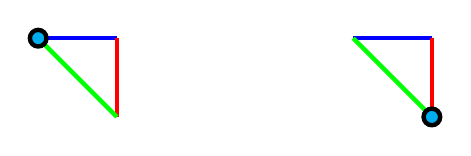
\begin{tikzpicture}

\begin{scope}[shift={(-2,0)}]
    \draw[ultra thick, blue] (-1,0) -- (0,0);
    \draw[ultra thick, red] (0,0) -- (0,-1);
    \draw[ultra thick, green] (0,-1) -- (-1,0);

    \node[style={circle, fill=cyan, draw, ultra thick, minimum size = 6pt, inner sep=0pt}] at (-1,0) {};
\end{scope}

\begin{scope}[shift={(2,0)}]
    \draw[ultra thick, blue] (-1,0) -- (0,0);
    \draw[ultra thick, red] (0,0) -- (0,-1);
    \draw[ultra thick, green] (0,-1) -- (-1,0);

    \node[style={circle, fill=cyan, draw, ultra thick, minimum size = 6pt, inner sep=0pt}] at (0,-1) {};
\end{scope}

\end{tikzpicture}
\caption{The fundamental domains and generating vertices of a cube (left) and a octahedron (right)}
\end{figure}

\begin{figure}[!h]
\centering

\begin{tikzpicture}
    \begin{scope}[shift={(-2,0)}]
        \begin{scope}[every node/.style={circle, fill=white, draw, thick, minimum size = 10pt, inner sep=0pt}]
            \node (1) at (0,0) {};
        \end{scope}

        \begin{scope}[every node/.style={circle, fill=black, draw, thick, minimum size = 6pt, inner sep=0pt}]
            \node (1) at (0,0) {};
        \end{scope}
    \end{scope}

    \begin{scope}[shift={(2,0)}]

        \begin{scope}[every node/.style={circle, fill=black, draw, thick, minimum size = 6pt, inner sep=0pt}]
            \node (1) at (0,0) {};
        \end{scope}
    \end{scope}
\end{tikzpicture}
\caption{An active reflection (left) and and inactive reflection (right)}
\end{figure}

\begin{figure}[!h]
\centering
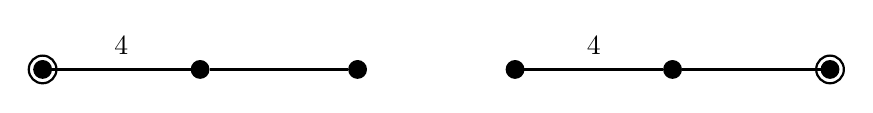
\begin{tikzpicture}
    \begin{scope}[shift={(-3,0)}]
        \begin{scope}[every node/.style={circle, fill=white, draw, thick, minimum size = 10pt, inner sep=0pt}]
            \node (1) at (0,0) {};
        \end{scope}

        \begin{scope}[every node/.style={circle, fill=black, draw, thick, minimum size = 6pt, inner sep=0pt}]
            \node (1) at (0,0) {};
            \node (2) at (2,0) {};
            \node (3) at (4,0) {};
        \end{scope}

        \begin{scope}[every edge/.style={draw,very thick}]
            \path [-] (1) edge (2);
            \path [-] (2) edge (3);
            \node at (1,0.3) {$4$};
            \node at (3,0.3) {};
        \end{scope}
    \end{scope}

    \begin{scope}[shift={(3,0)}]
        \begin{scope}[every node/.style={circle, fill=white, draw, thick, minimum size = 10pt, inner sep=0pt}]
            \node (1) at (4,0) {};
        \end{scope}

        \begin{scope}[every node/.style={circle, fill=black, draw, thick, minimum size = 6pt, inner sep=0pt}]
            \node (1) at (0,0) {};
            \node (2) at (2,0) {};
            \node (3) at (4,0) {};
        \end{scope}

        \begin{scope}[every edge/.style={draw,very thick}]
            \path [-] (1) edge (2);
            \path [-] (2) edge (3);
            \node at (1,0.3) {$4$};
            \node at (3,0.3) {};
        \end{scope}
    \end{scope}
\end{tikzpicture}
\caption{Extended Coxeter diagrams of a cube (left) and an octahedron (right)}
\end{figure}

We now have a way to represent different polytopes with the same Coxeter group using Coxeter diagrams. This can be used to differentiate between dual polytopes, but there are many other uniform polytopes with the same Coxeter group.

\subsection{Rectification}

\noindent\textbf{Definition 5.4.1.} \textit{Rectification} is the process of creating vertices at the midpoints of the edges of a polytope and connecting vertices on adjacent edges of the polytope.\newline

\begin{figure}[ht]
    \centering
    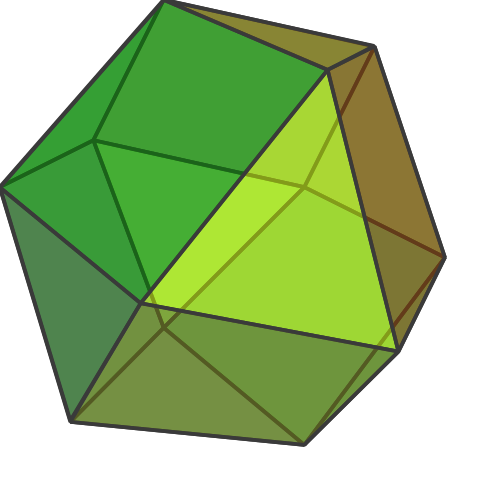
\includegraphics[width=0.2\textwidth]{uniform/Cuboctahedron.png}
    \caption{A rectified cube}
    \label{}
\end{figure}

\noindent\textbf{Definition 5.4.2.} A non-regular polytope is called \textit{quasiregular} if it's vertex-transitive, edge-transitive, and has regular faces.\newline

\noindent\textbf{Proposition 5.4.3.} The rectification of a regular or quasiregular polytope is uniform.
\begin{proof}
    Rectification turns edges into vertices. Therefore, a rectified polytope is vertex-transitive if and only if the original polytope is edge-transitive. Additionally, its faces are uniform if and only if the original polytope is edge-transitive.
\end{proof}

\noindent\textbf{Definition 5.4.4.} \textit{$k$-rectification} is the process of creating vertices at the midpoints of the $k$-faces of a polytope and connecting vertices on adjacent $k$-faces of the polytope.\newline

\noindent\textbf{Remark 5.4.5.} As we've seen, the dual of a polyhedron has vertices at its faces and faces at its vertices, meaning that 2-rectification (also called birectification) produces the dual of a polyhedron. In higher dimensions, $(k-1)$-rectification produces the dual of a $k$-polytope.\newline

\noindent\textbf{Corollary 5.4.6.} The $k$-rectification of a $k$-face-transitive polytope is uniform.\newline

This proof is the same as for Proposition 5.4.3 but with higher-dimensional faces.\newline

\noindent\textbf{Remark 5.4.7.} The rectification of a non-self-dual regular or quasiregular polytope has the same Coxeter group as that polytope. In extended Coxeter diagrams, $k$-rectification makes active nodes inactive, and makes nodes $k$ away from active nodes active.

\begin{figure}[!h]
\centering
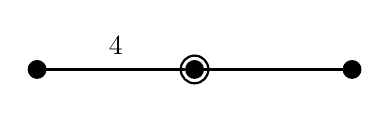
\begin{tikzpicture}
    \begin{scope}[every node/.style={circle, fill=white, draw, thick, minimum size = 10pt, inner sep=0pt}]
        \node (1) at (2,0) {};
    \end{scope}

    \begin{scope}[every node/.style={circle, fill=black, draw, thick, minimum size = 6pt, inner sep=0pt}]
        \node (1) at (0,0) {};
        \node (2) at (2,0) {};
        \node (3) at (4,0) {};
    \end{scope}

    \begin{scope}[every edge/.style={draw,very thick}]
        \path [-] (1) edge (2);
        \path [-] (2) edge (3);
        \node at (1,0.3) {$4$};
        \node at (3,0.3) {};
    \end{scope}
\end{tikzpicture}
\caption{Extended Coxeter diagram of the rectified cube}
\end{figure}

\subsection{Truncation}

\noindent\textbf{Definition 5.5.1.} \textit{Truncation} is the process of "cutting" the vertices of a polytope. This is done by removing the vertices of the polytope and creating a new facet in its place, bounded by the lines between equidistant points on adjacent edges. It is possible to "cut" the vertices by any amount, but \textit{uniform truncation} truncates such that all edges are the same length\footnote{This is not always possible for general polytopes.} (and all original edges still exist).\newline

\begin{figure}[ht]
    \centering
    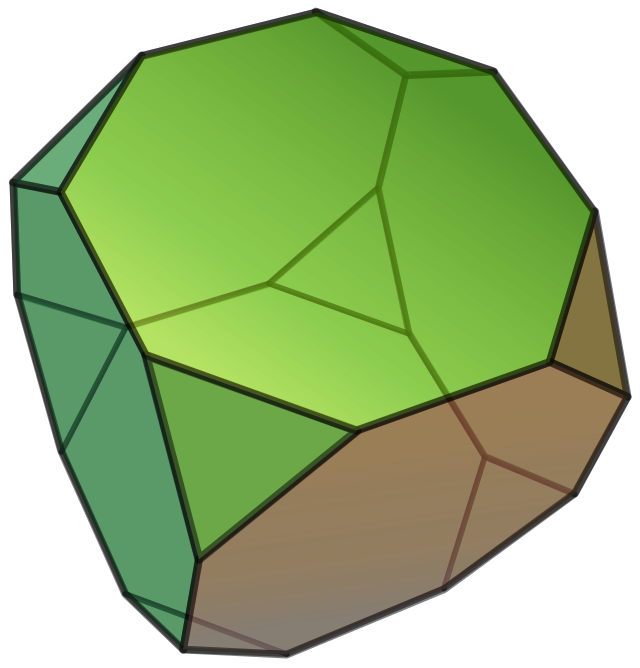
\includegraphics[width=0.2\textwidth]{uniform/Truncated_cube.png}
    \caption{A uniformly truncated cube}
    \label{}
\end{figure}

\noindent\textbf{Remark 5.5.2.} Truncating a quasiregular polytope using the midpoints of the edges as the boundary points defining the new facets is the same as rectification.\newline

\noindent\textbf{Proposition 5.5.3.} The uniform truncation of a uniform polytope with a uniform vertex figure is uniform.
\begin{proof}
    Truncation creates facets from the vertex figure of a polytope so the vertex figure must be uniform. Uniform truncation ensures that the truncated polytope is vertex-transitive.
\end{proof}

\noindent\textbf{Definition 5.5.4.} \textit{$k$-truncation} is the process of "cutting" the $j$-faces of a polytope $\forall j<k$. It can also be seen as expanding the polytope's $k$-faces (moving them directly away from its center and connecting previously adjacent $j$-faces with $(j+1)$-faces $\forall j<k$. As before, \textit{uniform $k$-truncation} creates a polytope with uniform facets.\newline

\noindent\textbf{Remark 5.5.5.} $2$-truncating a regular polytope is the same as rectifying its rectification\footnote{This can be seen more easily with extended Coxeter diagrams.}.\newline

\noindent\textbf{Definition 5.5.6.} Truncations can be combined to create a new transformation, \textit{$(k_1,k_2,...,k_m)$-truncation}. It "cuts" $k_i$-faces $\forall i \in \{1,...,m\}$. This can be seen as expanding a polytope's $k_1$-faces, then expanding its $k_2$-faces, and so on. \newline

\noindent\textbf{Remark 5.5.7.} The $(k_1,k_2,...,k_m)$-truncation of a regular polytope has the same Coxeter group as that polytope. In extended Coxeter diagrams, $(k_1,k_2,...,k_m)$-truncation makes nodes $(k_1,k_2,...,k_m)$ away from active nodes active.\newline

\begin{figure}[!h]
\centering
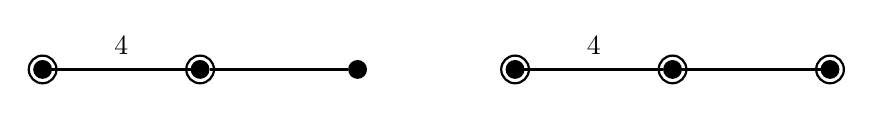
\begin{tikzpicture}
    \begin{scope}[shift={(-3,0)}]
        \begin{scope}[every node/.style={circle, fill=white, draw, thick, minimum size = 10pt, inner sep=0pt}]
            \node (1) at (0,0) {};
            \node (2) at (2,0) {};
        \end{scope}

        \begin{scope}[every node/.style={circle, fill=black, draw, thick, minimum size = 6pt, inner sep=0pt}]
            \node (1) at (0,0) {};
            \node (2) at (2,0) {};
            \node (3) at (4,0) {};
        \end{scope}

        \begin{scope}[every edge/.style={draw,very thick}]
            \path [-] (1) edge (2);
            \path [-] (2) edge (3);
            \node at (1,0.3) {$4$};
            \node at (3,0.3) {};
        \end{scope}
    \end{scope}

    \begin{scope}[shift={(3,0)}]
        \begin{scope}[every node/.style={circle, fill=white, draw, thick, minimum size = 10pt, inner sep=0pt}]
            \node (1) at (0,0) {};
            \node (2) at (2,0) {};
            \node (3) at (4,0) {};
        \end{scope}

        \begin{scope}[every node/.style={circle, fill=black, draw, thick, minimum size = 6pt, inner sep=0pt}]
            \node (1) at (0,0) {};
            \node (2) at (2,0) {};
            \node (3) at (4,0) {};
        \end{scope}

        \begin{scope}[every edge/.style={draw,very thick}]
            \path [-] (1) edge (2);
            \path [-] (2) edge (3);
            \node at (1,0.3) {$4$};
            \node at (3,0.3) {};
        \end{scope}
    \end{scope}
\end{tikzpicture}
\caption{Extended Coxeter diagrams of the truncated cube (left) and $(1,2)$-truncated cube (right)}
\end{figure}

\subsection{Alternation}

\noindent\textbf{Definition 5.6.1.} \textit{Alternation} is the process of removing every other vertex from a polytope and connecting vertices on previously adjacent edges. It is only possible to alternate polytopes with even-sided faces.\newline

\noindent\textbf{Definition 5.6.2.} The $k$-demicube is the alternated $k$-cube.\newline

\begin{figure}[ht]
    \centering
    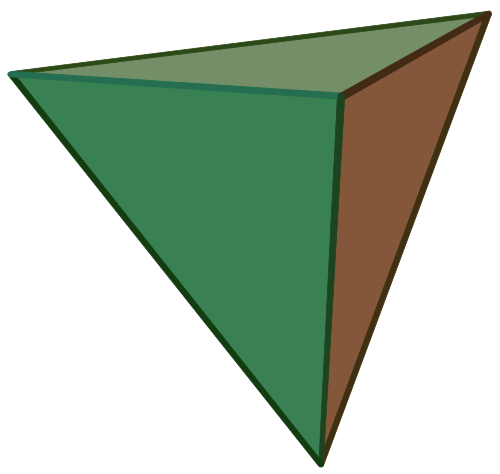
\includegraphics[width=0.2\textwidth]{uniform/Tetrahedron.png}
    \caption{A $3$-demicube (tetrahedron)}
    \label{}
\end{figure}

\noindent\textbf{Remark 5.6.3.} $D_n$ defines the $n$-demicube.\newline

\noindent\textbf{Definition 5.6.4.} An active reflection in a polytope's Coxeter group is called \textit{alternated} if the vertices generated by this reflection have been removed from the polytope. Alternated reflections are denoted with holes in extended Coxeter diagrams\footnote{These processes do not necessarily define unique polytopes, so neither do the extended Coxeter diagrams, however each extended Coxeter diagram only defines one polytope.}.\newline

\begin{figure}[!h]
\centering

\begin{tikzpicture}
    \begin{scope}[every node/.style={circle, fill=white, draw, thick, minimum size = 10pt, inner sep=0pt}]
        \node (1) at (0,0) {};
    \end{scope}
\end{tikzpicture}
\caption{An alternated reflection}
\end{figure}

\begin{figure}[!h]
\centering
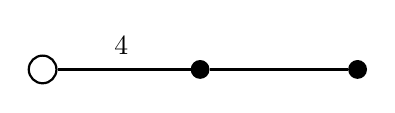
\begin{tikzpicture}
    \begin{scope}[every node/.style={circle, fill=white, draw, thick, minimum size = 10pt, inner sep=0pt}]
        \node (1) at (0,0) {};
    \end{scope}

    \begin{scope}[every node/.style={circle, fill=black, draw, thick, minimum size = 6pt, inner sep=0pt}]
        \node (2) at (2,0) {};
        \node (3) at (4,0) {};
    \end{scope}

    \begin{scope}[every edge/.style={draw,very thick}]
        \path [-] (1) edge (2);
        \path [-] (2) edge (3);
        \node at (1,0.3) {$4$};
        \node at (3,0.3) {};
    \end{scope}
\end{tikzpicture}
\caption{Extended Coxeter diagram of the $3$-demicube}
\end{figure}

\noindent\textbf{Theorem 5.6.5.} Every finite Coxeter group defines a uniform polytope.
\begin{proof}
    We will prove this by induction on the number of dimensions. In 2 dimensions, $I_2(m)$ defines the regular $m$-gon for $m\geq3$, which are all uniform. In $k$ dimensions, every finite Coxeter group that defines a $k$-polytope can be made by adding a new reflection to a finite Coxeter group that defines a $(k-1)$-polytope (equivalent to adding a node to a Coxeter diagram). By the induction hypothesis, this group defines a uniform $(k-1)$-polytope. Therefore, this polytope has a generating vertex in its ($(k-1)$-dimensional) fundamental domain. The $k$-dimensional fundamental domain (with the added reflection) contains the $(k-1)$-dimensional fundamental domain and so this vertex is the generating vertex of a (not necessarily uniform) n-polytope. We can move this vertex in the $k$th dimension while preserving the uniform $(k-1)$-polytope that it generates. Moving the vertex onto the new plane of reflection generates a polytope with uniform facets. Generating a polytope in this way creates a vertex-transitive polytope.
\end{proof}

\end{document}